\documentclass{beamer}

\usepackage[clean,pdf]{svg}
\usepackage{wrapfig}
\usepackage{hyperref}

\title{A Kochen-Specker system has at least 21 vertices}

\author{%
    \texorpdfstring{
        \begin{columns}%
            \column{.40\linewidth}
            \centering
            Sander Uijlen\\
            \texttt{suijlen@cs.ru.nl}
            \column{.40\linewidth}
            \centering
            Bas Westerbaan\\
            \texttt{bwesterb@cs.ru.nl}
        \end{columns}
    }{Sander Uijlen \& Bas Westerbaan}}

\institute{Radboud Universiteit Nijmegen}

% we don't want those funny buttons down right.
\setbeamertemplate{navigation symbols}{}

\begin{document}

\begin{frame}
    \titlepage
\end{frame}

\begin{frame}{}
        A \alert{Kochen-Specker system} $S$ is a finite set
        of points on the (open) northern hemisphere,
        such that there is no~$010$-coloring; that is: there is no~
        $\{0,1\}$-valued coloring with
        \begin{enumerate}
            \item
                three pairwise orthogonal points are assigned~$(1,0,0)$,
                        $(0,1,0)$ or~$(0,0,1)$ and
            \item
                two orthogonal points are not assigned~$(1,1)$.
                \\~\\
        \end{enumerate}
    \begin{tabular}{ll}
        point & $\sim$ direction of magnetic field
                    in measurement of SPIN-1 \\
        coloring & $\sim$ non-contextual deterministic theory
    \end{tabular}
    \pause
    \begin{theorem}[Kochen-Specker]
        There is a Kochen-Specker system.  Thus:
        there is no non-contextual deterministic theory
        predicting the measurement
        of a SPIN-1 particle.
    \end{theorem}
\end{frame}

\begin{frame}{The smallest Kochen-Specker system?}
    \begin{tabular}{lrl}
        Kochen-Specker & 1975 & $\leq 117$ \\
        Penrose, Peres (indep.) & 1991 & \onslide<2->{$\leq 33$} \\
        Conway & $\sim$ 1995 & \onslide<3->{$\leq 31$} \\
               & & \\
        \onslide<6->{U\&W}       & \onslide<6->{july?}&
                \onslide<6->{$\geq 22$ or $=21$} \\
        \onslide<5->{U\&W}       & \onslide<5->{may}& \onslide<5->{$\geq 21$} \\
                Arends, Wampler, Oauknine & 2009 &\onslide<4->{$\geq 18$} 
    \end{tabular}
\end{frame}

\begin{frame}{Conway's record}
    \begin{center}
        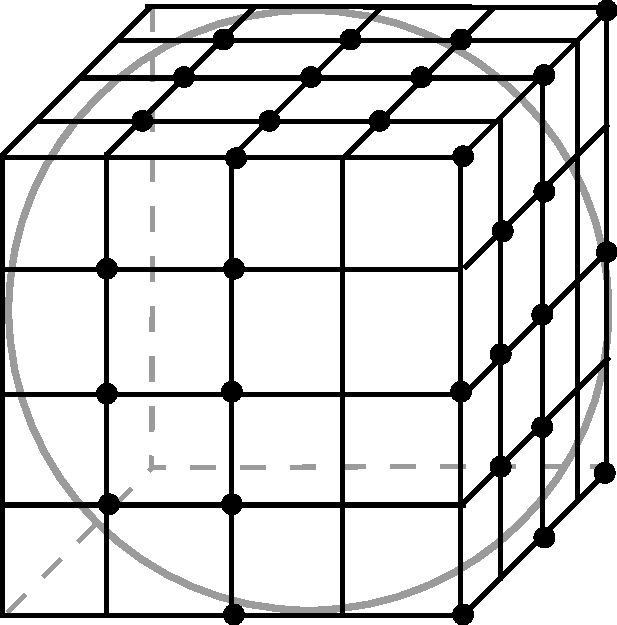
\includegraphics[width=7cm]{../graphs/ks31.pdf}
    \end{center}
\end{frame}

\begin{frame}{It is a problem about graphs}
    Given a finite set of points~$S$ on the projective plane,
    its \alert{orthogonality graph}~$\mathcal{G}(S)$
    has as vertices the points
    and two points are adjacent if and only if they are orthogonal.
    \pause
    \\~\\
    A graph~$G$ is \alert{embeddable}
    if there is a~$S$
    such that~$G \leq \mathcal{G}(S)$.
    \pause
    \\~\\
    A \alert{$010$-coloring} of a graph, is a~$\{0,1\}$-vertex coloring,
    such that
    \begin{enumerate}
        \item every triangle is colored~$(1,0,0)$, $(0,1,0)$ or~$(0,0,1)$ and
        \item no adjacent vertices are colored both~$1$.
    \end{enumerate}
\end{frame}

\begin{frame}{It is a problem about graphs}
    \begin{center}
    There is a Kochen-Specker system with~$n$ points \\
    if and only if \\
    there is a \alert{embeddable} and \alert{non-$010$-colorable}
            graph on~$n$ vertices.
    \end{center}
\end{frame}

\begin{frame}{Restrict the search}
    (The orthogonality graph of) a minimal Kochen-Specker system is
    \onslide<2>{
    \begin{wrapfigure}{r}{0.30\textwidth}
    \vspace*{-1cm}
        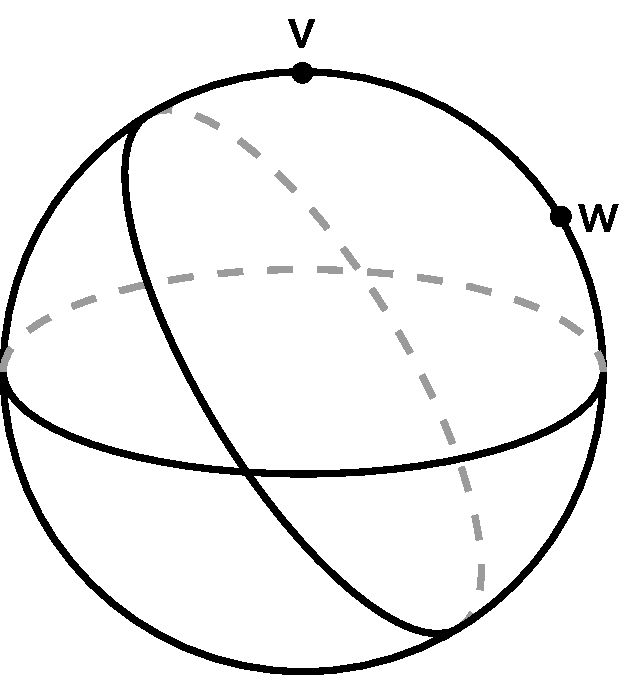
\includegraphics[width=0.30\textwidth]{../graphs/kruisproduct.pdf}
    \end{wrapfigure}}
    \begin{tabular}{ll}
        \onslide<1->{connected;} &
            \onslide<1->{$\sim 10^{26.4}$} \\
        \onslide<2->{squarefree and} &
            \onslide<2->{$\sim 10^{10.2}$} \\
        \onslide<3->{has minimal vertex degree 3;} &
            \onslide<3->{$\sim 10^{7.5}$} \\
    \end{tabular}
\end{frame}

\begin{frame}{The candidates}
Our computation found
the following number of
non $010$-colorable
squarefree graphs
with minimal vertex degree~$3$
\begin{center}
    \begin{tabular}{rl}
        $\#V$ & $\#$ candidates \\
        \hline
        $\leq 16$ & $0$ \\
        $17$ & $1$ \\
        $18$ & $2$ \\
        $19$ & $19$ \\
        $20$ & $441$ \\
        \onslide<2->{$21$} & \onslide<2->{$\geq 7616$}
    \end{tabular}
\end{center}
\end{frame}

\begin{frame}{Unembeddable subgraphs}
    All these candidates contain as a subgraph one of these
    unembeddable graphs.
    \begin{center}
    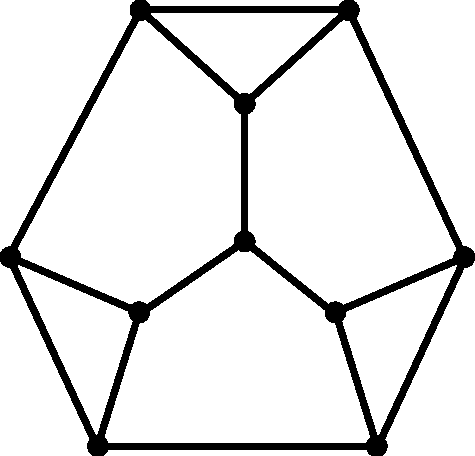
\includegraphics[width=3cm]{../graphs/unemb10-1.pdf}\qquad
    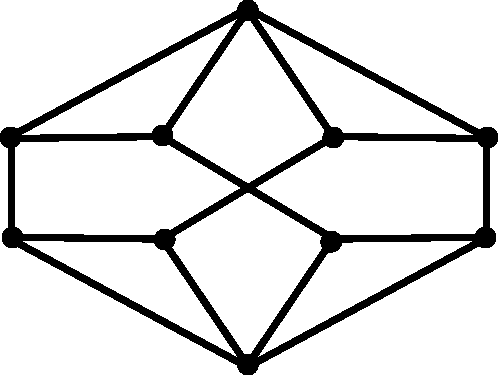
\includegraphics[width=3cm]{../graphs/unemb10-2.pdf}\qquad
    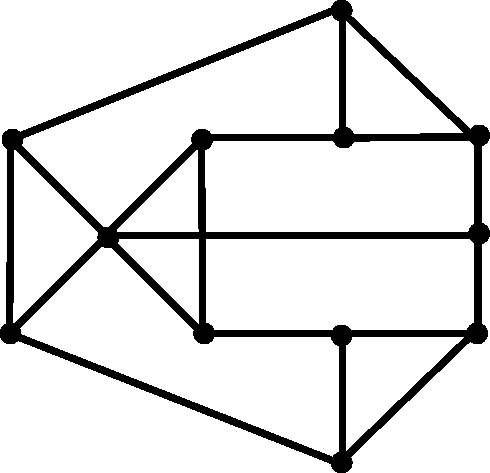
\includegraphics[width=3cm]{../graphs/unemb10-3.pdf}
    \end{center}
\end{frame}

\begin{frame}{Pen and paper proof of unembeddability}
    \begin{wrapfigure}{l}{0.33\textwidth}
        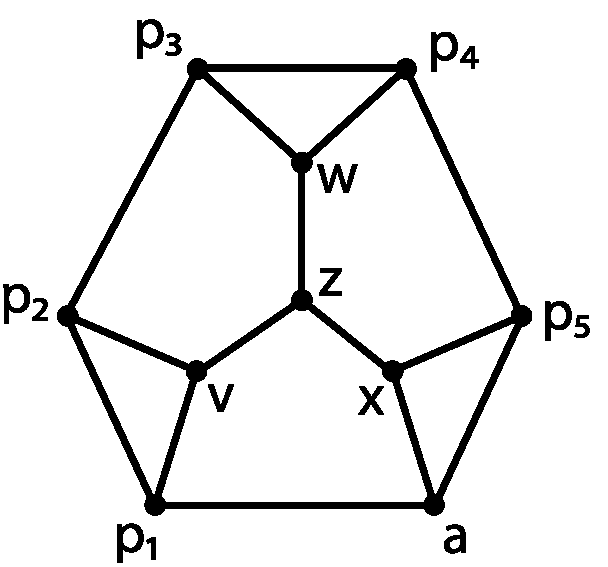
\includegraphics[width=0.35\textwidth]{../graphs/unemb10-1-a.pdf}
    \end{wrapfigure}
Suppose this graph is embeddable.
\\~\\

Note that~$v$ and~$a$ are distinct points orthogonal to~$p_1$.
Thus~$p_1$ is fixed.
Observe: $p_1$ is collinear to~$v \times a$.
\pause
\\~\\
Similarly: $p_2$ is collinear to~$v \times (v \times a)$.
And so on.  We see 
$a$ is collinear to $x \times (x \times (w \times (w \times (v \times
                    (v \times a)))))$.
\end{frame}

\begin{frame}{Pen and paper proof of unembeddability}
We may assume~$z=(0,0,1)$, $x=(1,0,0)$, $v=(v_1, v_2, 0)$, $w=(w_1,w_2,0)$
    and~$a=(0,a_2,a_3)$. We have:
\begin{equation*}
 \left(
\begin{smallmatrix}
0\\
a_2\\
a_3\\
\end{smallmatrix}
\right)
\text{is collinear to}
\left(
\begin{smallmatrix}
0\\
-a_2 v_1w_2 (v_1w_1 + v_2w_2) \\
-a_3 (v_1^2 w_1^2 + v_1^2 w_2^2 + v_2^2w_1^2 + v_2^2w_2^2)\\
\end{smallmatrix}
\right)
\end{equation*}
\pause
That is:
\begin{align*}
v_1w_2 \left<v,w\right> & =
v_1w_2 (v_1w_1 + v_2w_2) \\
& = v_1^2 w_1^2 + v_1^2 w_2^2 + v_2^2w_1^2 + v_2^2w_2^2 \\
& = (v_1^2 + v_2^2)w_1^2 + (v_1^2 + v_2^2)w_2^2 \\
& = w_1^2 + w_2^2 = 1.
\end{align*}
\pause
Since~$v$ and~$w$ are not collinear,
we have by Cauchy-Schwarz $|\left<v,w\right>| < 1$.
Note~$|v_1|, |w_2| \leq 1$.
Thus: $|v_1w_2\left<v,w\right>| < 1$.
Contradiction.
\end{frame}

\begin{frame}[fragile]{Example of automized cross product chasing}
    \fontsize{2}{1}
\begin{verbatim}
load_package redlog;
rlset R;

procedure d(x,y);
    (first x) * (first y) +
    (second x) * (second y) +
    (third x) * (third y);

procedure k(x,y);
    {(second x)*(third y) - (third x)*(second y),
     (third x)*(first y) - (first x)*(third y),
     (first x)*(second y) - (second x)*(first y)};

v0c1 := 1; v0c2 := 0; v0c3 := 0;
v1c1 := 0; v1c2 := 1; v1c3 := 0;

v0 := {v0c1, v0c2, v0c3}; 
v1 := {v1c1, v1c2, v1c3}; 
v2 := {v2c1, v2c2, v2c3}; 
v3 := {v3c1, v3c2, v3c3}; 
v2c1 := 0;
neq0 := k(v0,k(v3,v1)); 
\end{verbatim}
\begin{center} \emph{(snip)} \end{center}
\begin{verbatim}
neq29 := k(k(k(k(v3,v1),v1),v2),k(k(v3,v0),v3)); 
phi := 
       (first neq0 neq 0 or
        second neq0 neq 0 or
        third neq0 neq 0) and 
\end{verbatim}
\begin{center} \emph{(snip)} \end{center}
\begin{verbatim}
       (first neq29 neq 0 or
        second neq29 neq 0 or
        third neq29 neq 0) and 
       d(v2,v0) = 0 and 
       d(k(k(v3,v0),v3),k(k(k(k(v3,v1),v1),v2),v2)) = 0 and 
        true;
rlqe ex(v3c3,
     ex(v3c2,
     ex(v3c1,
     ex(v2c3,
     ex(v2c2,phi)))));
\end{verbatim}
\end{frame}

\begin{frame}
    Source code, paper and experimental results can be found at
    \begin{center}
        \url{kochen-specker.info}
    \end{center}
    \pause
    Some open problems:
    \begin{itemize}
        \item
            If~$G$ is embeddable,
            is there a~$S$ such that~$G = \mathcal{G}(S)$.
        \item
            Is every embeddable graph,
            grid embeddable? That is: using points of the form
            $(\frac{x}{\sqrt{n}}, \frac{y}{\sqrt{n}}, \frac{z}{\sqrt{n}})$
            for~$x,y,z,n \in \mathbb{Z}$.
    \end{itemize}
\end{frame}

\end{document}

% vim: ft=tex.latex
